% %%%%%%%%%%%%%%%%%%%%%%%%%%%%%%%%%%%%%%%%%%%%%%%%%%%%%%%%%%%%%%%%%%%%%%%%%%%%
% Thesis Defence
% Section: Background
% %%%%%%%%%%%%%%%%%%%%%%%%%%%%%%%%%%%%%%%%%%%%%%%%%%%%%%%%%%%%%%%%%%%%%%%%%%%%

\section[Prérequis]{Prérequis et Problématique}

% \begin{frame}
%     SpMV

%     OP

%     reductions

%     irrégulières

%     scatter

%     formats creux CSC

%     matrices creuses

%     correspondance direct vs associatif : 1 schéma pour expliquer les 3 types

%     visu du problème dans cache classique (au niveau, voir ASAP)
% \end{frame}

% \begin{frame}
%     Cache : mémoire intermédiaire entre le processeur et la mémoire principale

%     Fonction : stocker quelques données proche du processeur

%     Pourquoi : une transaction en mémoire principale prend du temps ($\sim$100 ns)
% \end{frame}

\begin{frame}
    \frametitle{Les matrices creuses}

    Slide 1 de HiPEAC

\end{frame}

\begin{frame}
    \frametitle{Les matrices creuses jusqu'au problème dans cache, et intro SpDCache}

    Premières slides de ASAP

\end{frame}

\begin{frame}
    \frametitle{Les modèles développés pour étudier et évaluer SpDCache}

    Trois modèles :

    \bigskip\bigskip\bigskip\bigskip

    \begin{tblr}{
            width = {\linewidth},
            colspec = {X[1.2,c] *{3}{X[2,c]}}, % rowspec
            rows = {m},
            colsep = {4pt},
            row{1-Z} = {rowsep=2pt, black!2},
            row{1} = {c, font=\bfseries, black!5},
            hspan = {minimal},
            % hlines, vlines,
            % rulesep = {-1pt},
            hline{1,Z} = {2pt}, % Z for last
            hline{2} = {1pt},
            % hline{Z} = {1pt, dashed},
            vline{2-Y} = {1-Z}{0.5pt},
        }
        %
        Modèle & Modèle analytique & Modèle de simulation & Implémentation RTL \\
        Langage & C & Python & SystemVerilog \\
        Entrées & Distributions de densités & Matrices réelles et synthétiques & Matrices réelles et synthétiques \\
        Niveau de paramétrisation & Très élevé +++ & \'Elevé ++ & Moyen + \\
        Vitesse de simulation & $\sim$10\textsuperscript{5} $nnz/s$ +++ & $\sim$10\textsuperscript{3} $nnz/s$ ++ & $\sim$10 $nnz/s$ + \\
        Précision & Probabilité + & Transaction ++ & Cycle +++ \\
        Design & Approximatif & Exact & Exact avec contraintes matérielles \\
        %
    \end{tblr}

    \begin{tikzpicture}[remember picture, overlay]
        \node [shift={(-4.7cm, 1.70cm)}, rotate=5] at (current page.center)
            { 
\includegraphics[width=0.08\linewidth]{Figures/PDF/Sticker_C.pdf} };
    \end{tikzpicture}

    \begin{tikzpicture}[remember picture, overlay]
        \node [shift={(-0.7cm, 1.80cm)}, rotate=-5] at (current page.center)
            { 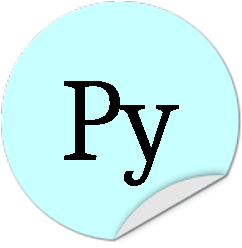
\includegraphics[width=0.08\linewidth]{Figures/PDF/Sticker_Py.pdf} };
    \end{tikzpicture}

    \begin{tikzpicture}[remember picture, overlay]
        \node [shift={(3.5cm, 1.73cm)}, rotate=7] at (current page.center)
            { 
\includegraphics[width=0.08\linewidth]{Figures/PDF/Sticker_RTL.pdf} };
    \end{tikzpicture}

\end{frame}

\begin{frame}
    Problème :

    Comment traiter efficacement des réductions irrégulières ?

    Deux approches complémentaires :

    Approche 1 : Cache de réduction pour calculer les réductions dans le cache et éviter des transactions inutiles

    Approche 2 : Traiter l'irrégularité en s'appuyant sur la structure des matrices, partitionnement du cache
\end{frame}